\chapter{Research}
\label{research}

\section{Data selection}
\label{method:data}
A total number of 250 OSS projects will be used for this study. This number is
somewhat arbitrary, but was chosen to have a much larger data set than the
initial study conducted by \citet{karus2013}, as we believe a larger data
set yields more trustworthy results, and still keep the research feasible
within the given time constraints of four months.

Several steps have been taken prior to the selection of this set of 250
projects. The steps are described in the following sections.

\subsection{Data gathering}
The data for this research is gathered from
Ohloh\footnote{\url{http://www.ohloh.net}}: \emph{``Ohloh is a free, public
directory of Free and Open Source Software and the contributors who create and
maintain it.'' }\rm \cite{ohloh}. At the time of this writing, Ohloh tracks more
than 660,000 OSS projects varying in all ranges of size, and popularity. The
most popular projects currently being Apache HTTP Server, Apache OpenOffice,
Apache Subversion, Bash, Firebug, Linux Kernel, Mozilla Firefox, MySQL, PHP,
and Ubuntu.

\paragraph{}
For this research, we use the data provided by a tool by \citet{ohlohanalytics}.
This tool, ``\emph{OhlohAnalytics}\rm'', was developed as part of the
replicative research by \citet{bruntink2014}, and provides a validated and
cleansed data set of 12,360 OSS projects, collected from Ohloh in July 2013.

\subsubsection{Initial validation and cleansing}
The OhlohAnalytics tool by \citet{ohlohanalytics} did the initial analysis,
validation, and cleansing of the data by detecting inconsistent values and
removing these records from the data set. Additionally, extra data fields are
derived or aggregated from and added to the raw data for convenience.

The complete list of data fields provided by OhlohAnalytics are shown in Table
\ref{table:fields}. The column 'Source' specifies if the field is either 'Raw'
data (i.e., directly available from Ohloh), or if it is added by the
OhlohAnalytics tool as derived from an operation on one or more other fields.
In the latter case, the fields are listed.

The result of the data gathering and cleansing step is a consistent data set of
evolution data of 10,811 projects.

\newcommand{\tableHeadDataFields}{\bfseries{Field}\rm & \bfseries{Source}\rm &
\bfseries{Description}\rm}
\begin{table}
	\caption{Monthly data fields}\label{table:fields}
	\begin{tabular}{p{4cm} p{3cm} p{7.5cm}}
		\hline
		\tableHeadDataFields \\ \hline
		
		project\_name\_fact & Raw & The name of the project at Ohloh. \\
		\hline
		
		\bfseries{Activity}\rm \\ \hline

		abs\_loc\_growth & $loc\_added\_fact$, $loc\_deleted\_fact$ & The number of
		'lines of code' (LOC) that the project has grown (or shrank) current month. \\

		blanks\_added\_fact & Raw & The number of blank lines added to source text
		current month. \\

		blanks\_deleted\_fact & Raw & The number of blank lines deleted from source
		text current month. \\

		comments\_added\_fact & Raw & The number of lines of comments added in source
		text current month. \\

		comments\_deleted\_fact & Raw & The number of lines deleted from source text
		which are comments; for current month. \\

		commits\_fact & Raw & The total number of commits made current month. \\

		contributors\_fact & Raw & The total number of contributors who made at least
		one commit current month. \\

		ind\_loc\_growth & $loc\_fact$, $abs\_loc\_growth$ & The relative growth of
		the project measured in LOC for current month. \\

		loc\_added\_fact & Raw & The number of LOC added current month. \\

		loc\_deleted\_fact & Raw & The number of LOC deleted current month. \\
		\hline
		
		\bfseries{Analysis}\rm \\ \hline

		age\_in\_months & $month\_fact$, $year\_fact$ & The age of the project in
		months measured since the first data point; starts at 0. \\

		age\_in\_years & $age\_in\_months$ & The age of the project in years measured
		since the first data point; starts at 0. \\

		cumulative\_commits\_fact & $commits\_fact$ & The total number of commits
		since the first data point (i.e., where $age\_in\_months = 0$). \\

		main\_language\_fact & Raw & The programming language having the highest LOC
		value for the project in current month (XML and HTML are ignored). \\

		month\_fact & Raw & The month value of current month's analysis. Extracted from
		$udpated\_at$ field. \\

		year\_fact & Raw & The year value of current month's analysis. Extracted from
		$updated\_at$ field. \\
		\hline
		
		\bfseries{Size}\rm \\ \hline

		blanks\_fact & Raw & The total number of blank lines in source text in current
		month. \\

		comment\_ratio\_fact & Raw & The fraction of net lines in source text which
		are comments; for current month. \\

		comments\_fact & Raw & The total number of lines in source text which are
		comments; for current month. \\

		loc\_fact & Raw & The total number of LOC current month. \\

		\hline
	\end{tabular}
\end{table}

\subsection{Data validation}
\subsubsection{Subsequent data series}
Although the data set should be consistent after validation and cleansing, we 
need another validation step prior to the selection of the 250 projects for the
study.

The evolution data of the 10,811 projects contained gaps. We expect a
subsequent series of data is necessary to be able to analyse time series for a
project. Therefore, a number representing the \emph{fraction of continuity }\rm
of the evolution data per project was needed. For each project the difference
between the minimum and maximum values of the $age\_in\_months$ fact is taken,
added by one, giving us the expected number of data points for a project. The
calculation of the fraction of total evolution data is done for each project.

After the fractions of the total evolution data for each project were caculated,
these projects were filtered and only the projects that have all data points
between minimum and maximum $age\_in\_months$ are kept. From the set of 10,811
projects, a total number of 6,418 projects is left.

\subsubsection{Minimal sequence length}
A time series of 1 (monthly) data point is obviously not analysable over time
and uncomparable to larger projects. The threshold of at least 12 monthly data
points is chosen to minimise noise in the evolution data that may be caused by
too young or unstable projects.

After this selection, a set of 5,986 projects is left.

\subsubsection{Representativeness}
For the selection of a sample of 250 projects, we use the tool created by
\citet{nagappan} at Microsoft Research. This tool takes a, possibly atomic,
sample set and selects additional projects to add to the sample that increase
the overall representativeness of that sample. The tool scores projects by two
metrics: total lines of code, and yearly contributors count.

The tool iteratively selects 250 projects and adds it to the sample. Each
additional project is selected by its score to maximally increase the
representativeness of the sample as a whole, compared to the master data.

The master data is a list of 20,028 projects tracked by Ohloh delivered with
this tool. A pre-filtering of this master data was done to make the tool select
only the projects that appear in our data set of 5,986 projects. After
pre-filtering, a subset of the master data of 1,588 projects is left. From this
subset, a sample of 250 projects was selected.

The resulting sample of 250 projects was scored against the initial master data
of 20,028 projects and scores a 99.5\% representativeness.

\subsection{Results}
The results of the Data selection phase of the study are the following: the
evolution data of 250 distinct projects having a total of 22,943 data points.
The biggest project having 321 monthly data points, the smallest having 14
monthly data points. This confirms that there are no projects with less
than 12 monthly data points.

\section{Wavelet transform and analysis}
\subsection{Project signals}
The evolution of the 250 projects are modeled as signals as input for the
wavelet transform and analysis. We have constructed project signals by modeling
$age\_in\_months$ in the time domain, and $LOC$ in the frequency domain. Figure
\ref{figure:signal} shows a project's signal.

\begin{figure}[H]
\caption{LOC signal of project \#19012}\label{figure:signal}
\centering
	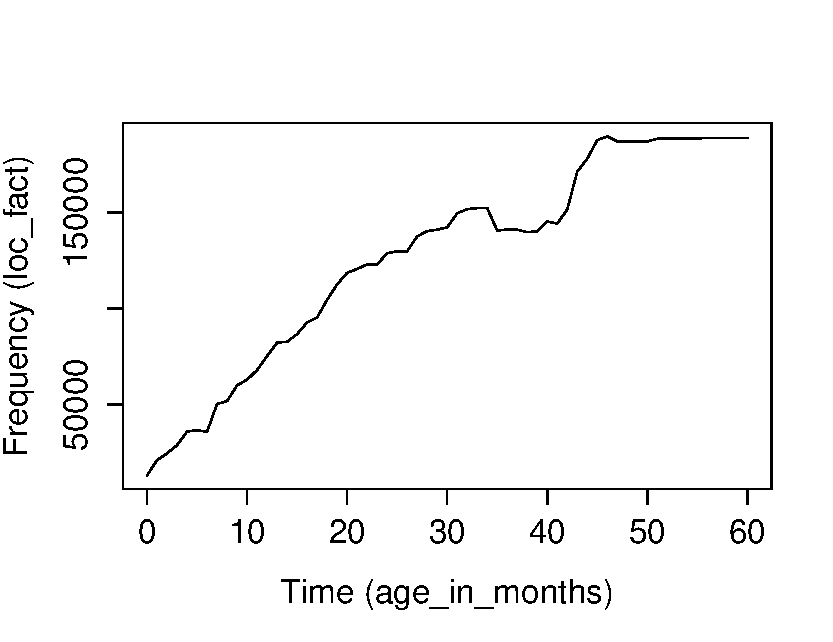
\includegraphics[height=192pt]{images/signal_pid_19012.pdf}
\end{figure}

\paragraph{}
The $LOC$ we used in the transform and analysis is slightly different from the
$loc\_fact$ that exists in the data set. The goal for the signal processing is
that we are able to detect patterns in a project's code activity. This means we
are interested in all changes that occur in source files. Therefore, we took
the same metric as in the original study by \citet{karus2013}. The $LOC$ metric
is constructed as the sum of $loc\_fact$, $comments\_fact$, and $blanks\_fact$.

\paragraph{}
For the wavelet transform and analysis, we have used R Statistics Suite
with packages ``wavelets'', ``chron'' and ``zoo''. The Wavelets package
contains a implementations of discrete wavelet transform functions, including
the Haar filter; Chron provides functions for working with chronological data
series; and Zoo eases indexing of and working with indexed data.

The Haar filter is used by \citet{karus2013} in his research because of its
simplicity and ease of interpretation. As this study is a replication of
\citeauthor{karus2013}' study, the choice of using the Haar filter was made.

\paragraph{}
The R scripts used for the steps of wavelet transform, sequence identification,
and grouping, are based on the scripts created and used by
\citeauthor{karus2013} in the initial research. Small adjustments have been
made to make the scripts compatible with our data set.

\subsection{Wavelet transform}
The first step in the analysis of time series of software evolution is the
wavelet transform. During this step discrete wavelet transform using the Haar
filter is applied on a project's signal. The results comprise the
coefficients\footnote{The coefficients are not the same as data points. The
data points represent monthly facts from a project, and the coefficients in
sequences represent values found at a certain level of decomposition from the
wavelet transform. More specifically: the coefficients are values resulted from
shifting or filtering the signal.} at each level of decomposition which are
saved for further analysis. For more details on this analysis method see
section \ref{wavelet_analysis}.

\subsection{Wavelet analysis}
\subsubsection{Similar sequence identification}
During this step the resulting coefficients from the wavelet transform are
analysed to find \emph{similar sequences}\rm. A sequence is defined as a
subsequent series of coefficients, at a particular level of decomposition, with
a sequence length between 3 and 65 (inclusive) coefficients.

The thresholds were chosen by \citet{karus2013} in the original study to
distinguish a sequence from an ordinary set of coefficients if the sequence is
very short (length 1 or 2). On the contrary, if a sequence is larger than 65 we
have to be able to distinguish the sequence from the complete signal.

A sequence is considered 'similar' if at least one other sequence was found of
which the values of the coefficients are equal with respect to an allowed
deviation. Similar sequences may be found within one project, but preferrably be
found across projects.

\paragraph{}
The similar sequence identification found 1,669,448 sequences that occurred
at least 2 times in the data. Only 16 sequences were found using wavelet/shift
coefficients, the other 1,669,432 sequences were found using filter/scale
coefficients.

\subsubsection{Similar sequence grouping}
\label{def:pattern}
Not all of the sequences found in the previous step are interesting. Many of
these sequences are just small changes in the signal. In this step, the similar
sequences from previous step are taken as input to find 'patterns'.

\paragraph{}
A sequence is considered a 'pattern' if it appears at least 3 times in the
sequence data. Each pattern is assigned an identification number to be used in
further analysis.

The sequences that are instances of the same pattern are grouped together and
added meta data, such as the number of occurrances, the list of projects
it occurs, and whether it appears in dead, alive, or both dead and alive
projects.

\subsection{Results}
The results of this step revealed a total of 16,049 patterns in the projects.
All the patterns were found in the sequences resulting from using filter
coefficients, and 0 in those from using wavelet coefficients. The sequences
occurred at least 4 times, and at most 1,511 times. They occur in at least 1
and at most 204 projects. Their lengths differ between 4 and 19 points across
various decomposition levels (levels of detail).

\section{Pattern identification}
\subsection{Dead project identification}
In the search to find patterns that are warning signs leading to the end of
code evolution, we first extract from our initial 250 projects the projects
that satisfy the definition of a dead project (see also section \ref{def:dead}).
A total of 43 projects are dead according to the definition and their evolution
data in the data set. However, further verification is needed to confirm that
these projects are indeed dead.

\paragraph{}
Our data set contains data points up to June 2013. After manual verification of
the 'dead' projects with data up to April 2014, we could confirm that 21 of the
43 projects have had no code activity in the period between June 2012 and
April 2014. This data is acquired by consulting the project's websites, source
code repositories and commit history, and the data available at Ohloh.

More information on the results of the evaluation of dead projects can be found
in section \ref{section:deads}.

\subsection{Patterns in dead projects}
Given this set of 21 dead projects, we can select all patterns occurring in
these dead projects. Patterns occurring in dead projects can be hints of
evolutionary events that lead to the death of a project.

A total number of 967 patterns were found across dead projects. The patterns
do not occur at the same moment in the lifetime of the projects. Therefore, we
have introduced different types of patterns for dead projects:

\begin{description}
	\item[Type A.] Type A patterns strictly occur at the end of the evolution data
		of a dead project. More formaly, if a dead project $P$ starts at point $x$ and
		ends at point $y$, the pattern starts at $x'$ and ends at $y$. In our data
		set, the maximum date $y$ of $P$ is June 2013.
	
	\item[Type B.] Type B patterns strictly \emph{do not }\rm occur at the end of
		evolution data of a dead project, but anywhere else in the lifetime of a dead
		project.
	
	\item[Type AB.] Type AB patterns are patterns that behave like both types A and
		B patterns.
\end{description}

\noindent
The above types partition the patterns into three disjunctive sets.

In the search for patterns that are warning signs, we are mostly interested in
patterns of type A, because these patterns could indicate an evolutionary event
that lead to the end of code evolution for the dead projects it appears in.

\subsection{Results}
From the 967 patterns that were found across 21 dead projects, 25 of these
patterns are type A patterns, 317 of type B, and 625 of type AB.


\begin{comment}
- Execution of the research
- Phases, steps

This chapter reports on the execution of the research method as described in Chapter 3.

If the research has been divided into phases (e.g., using sub questions) the
phases are introduced, reported on and concluded individually. If needed this
Chapter could be split up to balance out the sizes of all Chapters.
An example Research Chapter is provided as Chapter 3 at Paul’s home
page\footnote{http://homepages.cwi.nl/~paulk/thesesMasterSoftwareEngineering/2006/ReneWiegers.pdf}.
\end{comment}
